\section{State Diagrams}
Die \textbf{State Diagrams} in \textbf{Phase 2} werden benutzt, um das interne Verhalten der \textit{SmartWatch} bei ausgewählten Benutzerinteraktionen darzustellen. Die Diagramme definieren, das Verhalten und die Bearbeitung bei einzelnen Eingaben. Zu diesem Zeitpunkt der Entwicklungsphase wurden die Zustände für die \textit{Verbindung zum Smartphone} \textit{(Pairing)}, das Verwenden der \textit{Fitnessapplikationen} und deren \textit{Speicherfunktion}, sowie das Verhalten bei \textit{ein- und ausgehenden Anrufen} modelliert.\\
\begin{figure}[h]
\centering\
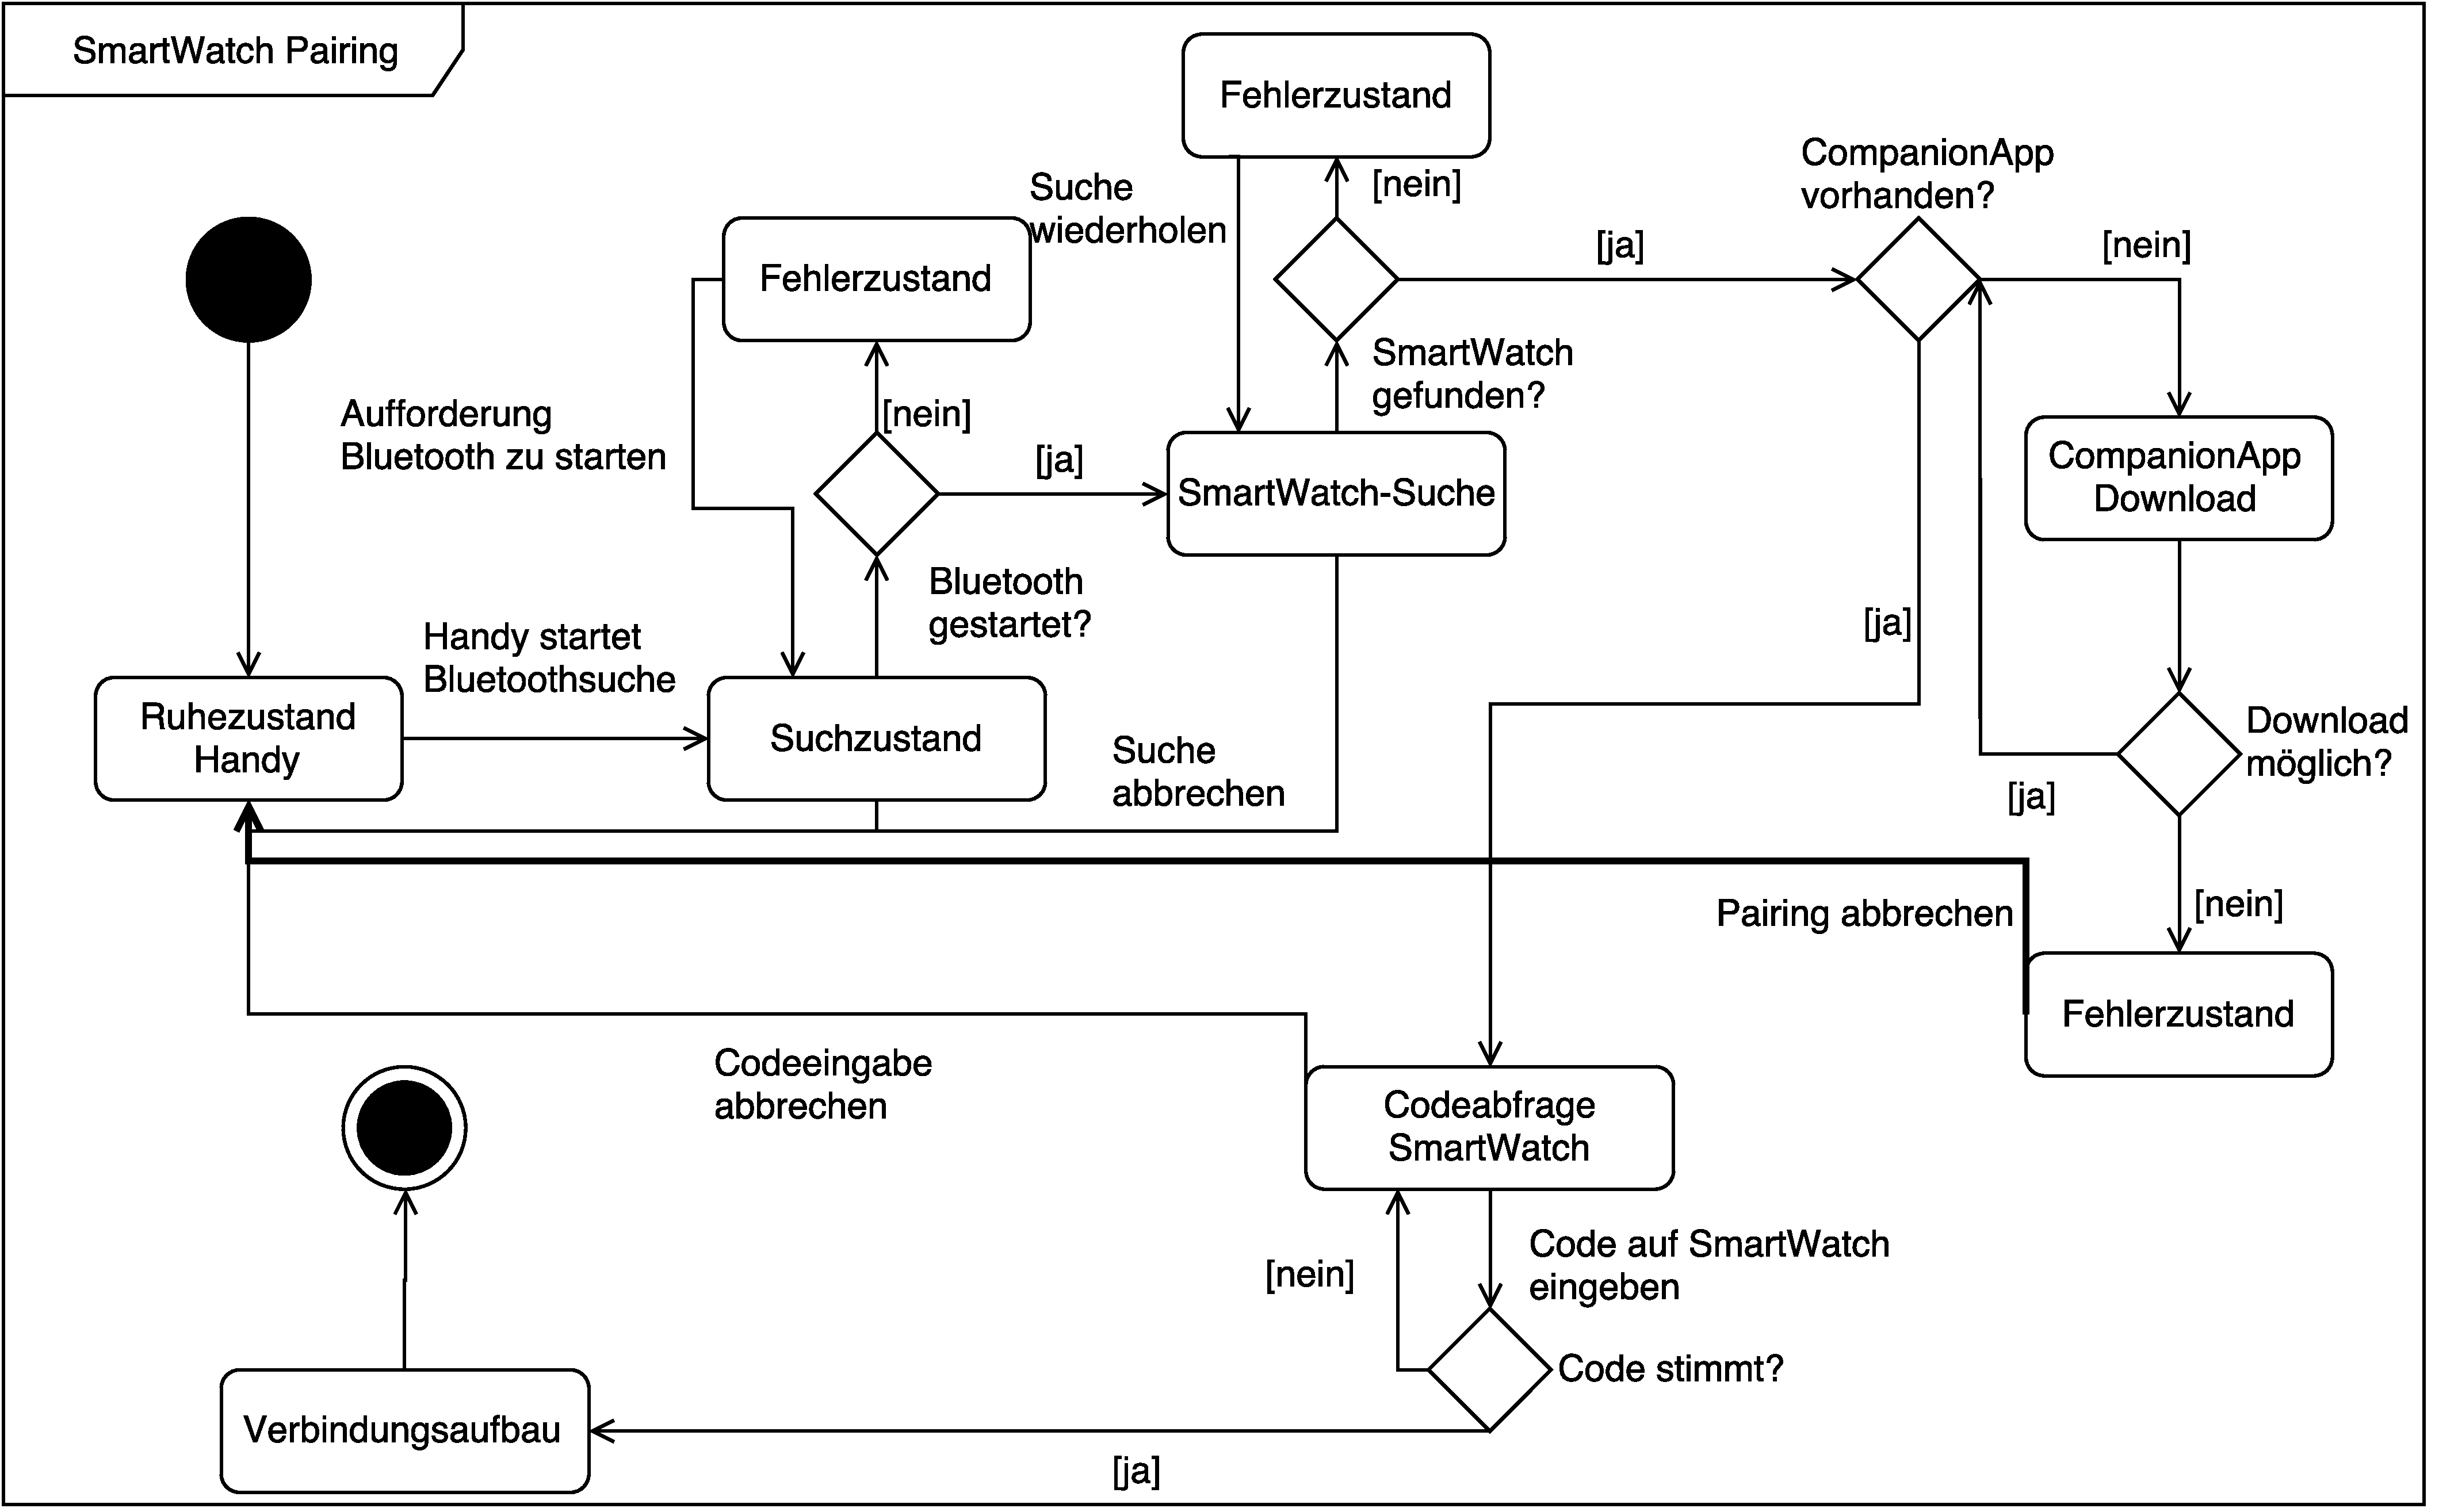
\includegraphics[width=\textwidth]{img/statePairing}
\caption[State Diagram: Pairing]{Verhalten der SmartWatch beim Pairing mit dem SmartPhone.}
\label{fig:statePairing}
\end{figure}
Wenn sich die \textit{SmartWatch} mit dem \textit{SmartPhone} verbinden soll, wird zunächst beim Handy mittels \textit{Bluetooth} nach der \textit{SmartWatch} gesucht. Dabei muss bei \textbf{beiden} Geräten das \textit{Bluetooth-Modul} aktiviert sein, da ansonsten keine Verbindung möglich ist. Wenn sich die Geräte gegenseitig gefunden haben, wird überprüft, ob sich auf dem \textit{SmartPhone} die zur \textit{SmartWatch} dazugehörige \textit{Companion-App} befindet. Sollte diese noch nicht installiert sein, wird der Benutzer dazu aufgefordert, dies zu tun, denn ohne die installierte \textit{Companion-App} ist ein \textit{Pairing} nicht möglich. Wenn die App funktionstüchtig ist, wird der Benutzer aufgefordert, den vom \textit{SmartPhone} generierten Code auf der \textit{SmartWatch} einzugeben. Dies dient dazu, dass sich nicht andere \textit{SmartPhones} willkürlich mit der \textit{SmartWatch} verbinden können. Wenn der Code erfolgreich eingegeben wurde, erfolgt die Verbindung zwischen beiden Geräten. Bei jedem der Schritte für den Verbindungsaufbau ist es möglich, den Vorgang abzubrechen und \textit{SmartPhone} und \textit{SmartWatch} in den Ruhenzustand zurückzuversetzen Abb. \ref{fig:statePairing}.\\
\begin{figure}[h]
\centering\
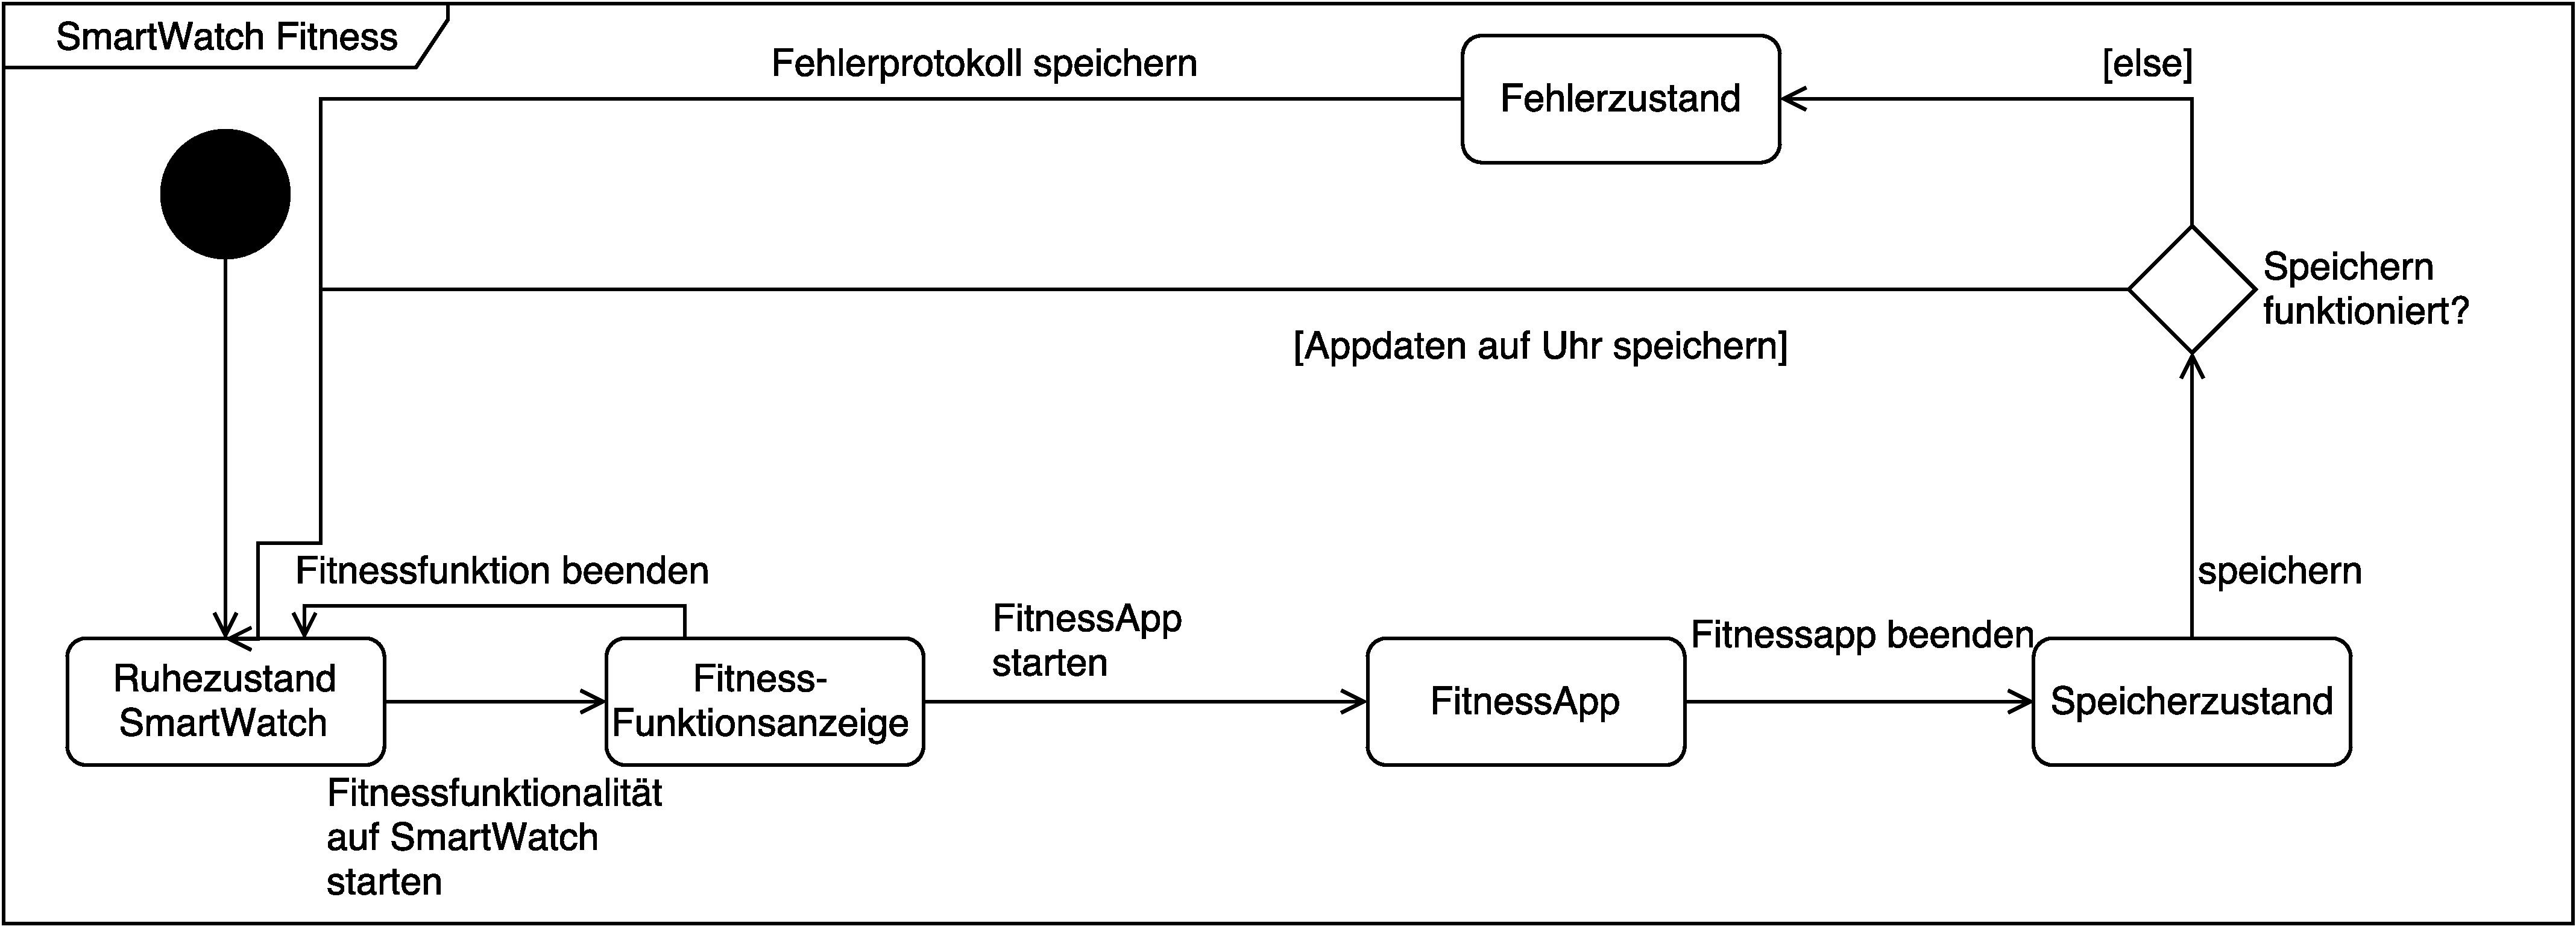
\includegraphics[width=\textwidth]{img/stateFitness}
\caption[State Diagram: Fitness]{Verhalten der SmartWatch beim Starten der Fitnessapp.}
\label{fig:stateFitness}
\end{figure}
Wenn die \textit{native Fitnessfunktionalität} der \textit{SmartWatch} benutzt werden soll, muss die Uhr zunächst aus dem Ruhezustand geholt werden. Anschließend wird über das Menü die \textit{Fitnessapp} ausgewählt, bestätigt und daraufhin die Routine zur Aktivitätsaufzeichnung ausgeführt. Sobald diese beendet ist, versucht die \textit{SmartWatch} die Fitnessdaten im \textit{internen Speicher} abzulegen. Wenn der \textit{Speichervorgang} erfolgreich war, werden die Daten auf dem internen Speicher abgelegt. Bei einem Fehler während des Speicherns, werden die Daten gelöscht und ein Fehlerprotokoll erstellt (Abb. \ref{fig:stateFitness}).\\
\begin{figure}[h]
\centering\
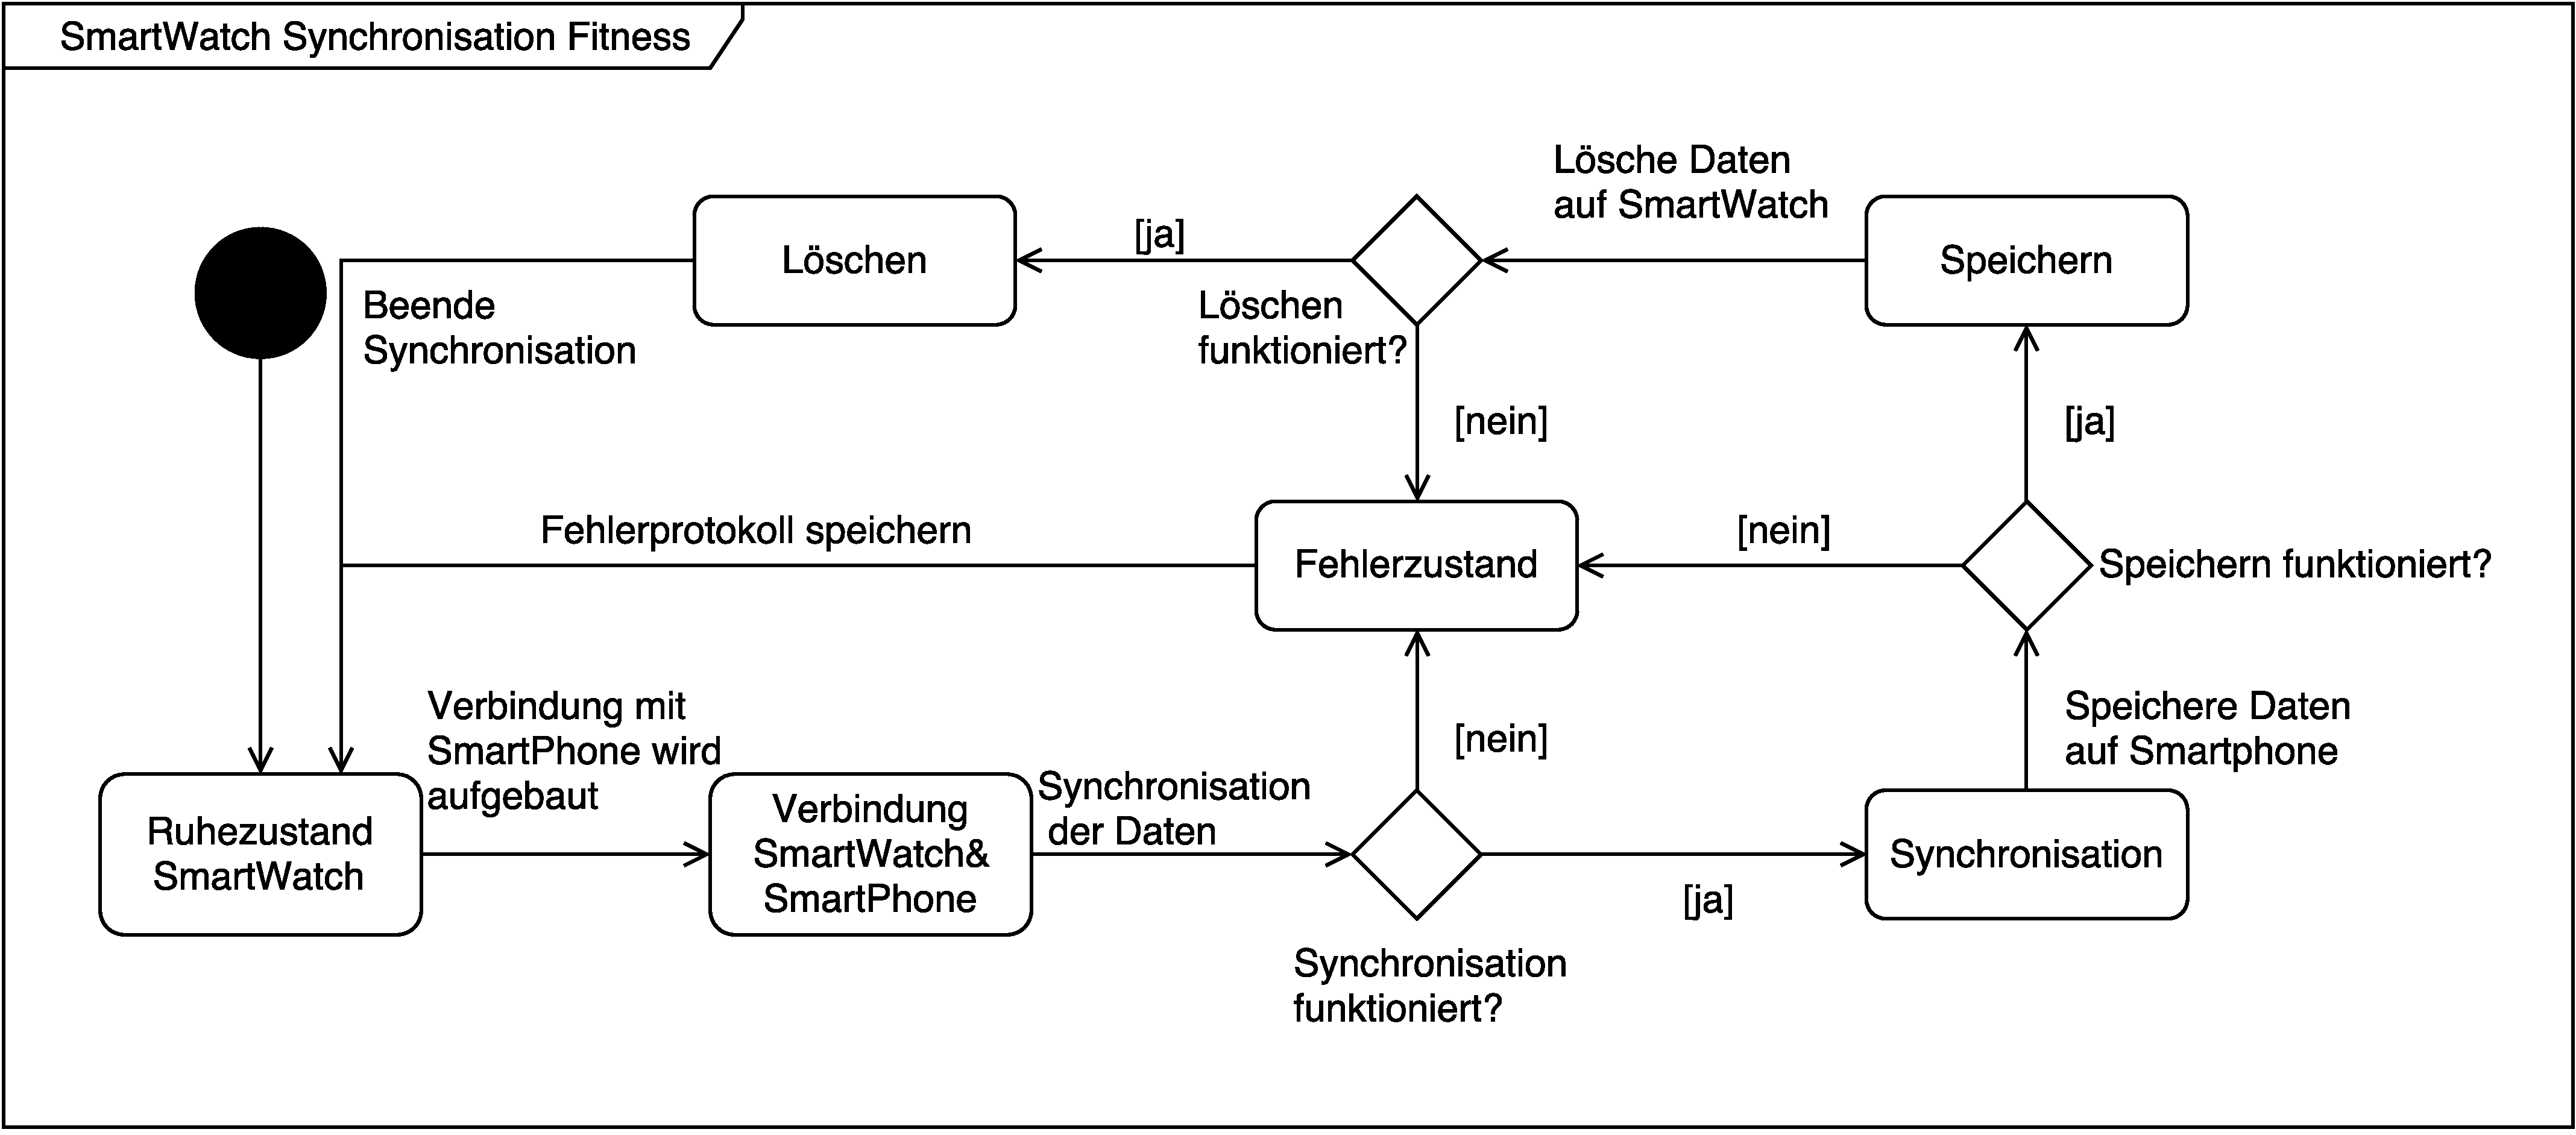
\includegraphics[width=\textwidth]{img/stateSync}
\caption[State Diagram: Synchronisation]{Verhalten der SmartWatch beim Synchronisieren der Fitnessaktivitäten mit dem SmartPhone.}
\label{fig:stateSync}
\end{figure}
Nachdem eine \textit{Fitnessaktivität} beendet und die \textit{Fitnessdaten} auf der \textit{SmartWatch} zwischengelagert wurden, wird versucht, bei der nächsten Verbindung, die \textit{Daten} von der \textit{SmartWatch} auf das \textit{SmartPhone} zu übertragen (Abb. \ref{fig:stateSync}). Voraussetzung dafür ist eine erfolgreiche \textit{Verbindung} zwischen den beiden Geräten. Sobald diese steht, wird mit dem \textit{Synchronisationsvorgang} begonnen. Bei folgendem werden zunächst die \textit{Daten} von der \textit{Uhr} auf das \textit{Telefon} gespeichert, um einen möglichen Datenverlust zu vermeiden. Anschließend werden die \textit{Daten} von der \textit{SmartWatch} gelöscht und die \textit{Synchronisation} beendet. Sollte im Verlauf der \textit{Synchronisation} ein Fehler auftreten, wird die \textit{Synchronisation} abgebrochen und ein \textit{Fehlerprotokoll} erstellt. \\
\begin{figure}[h]
\centering\
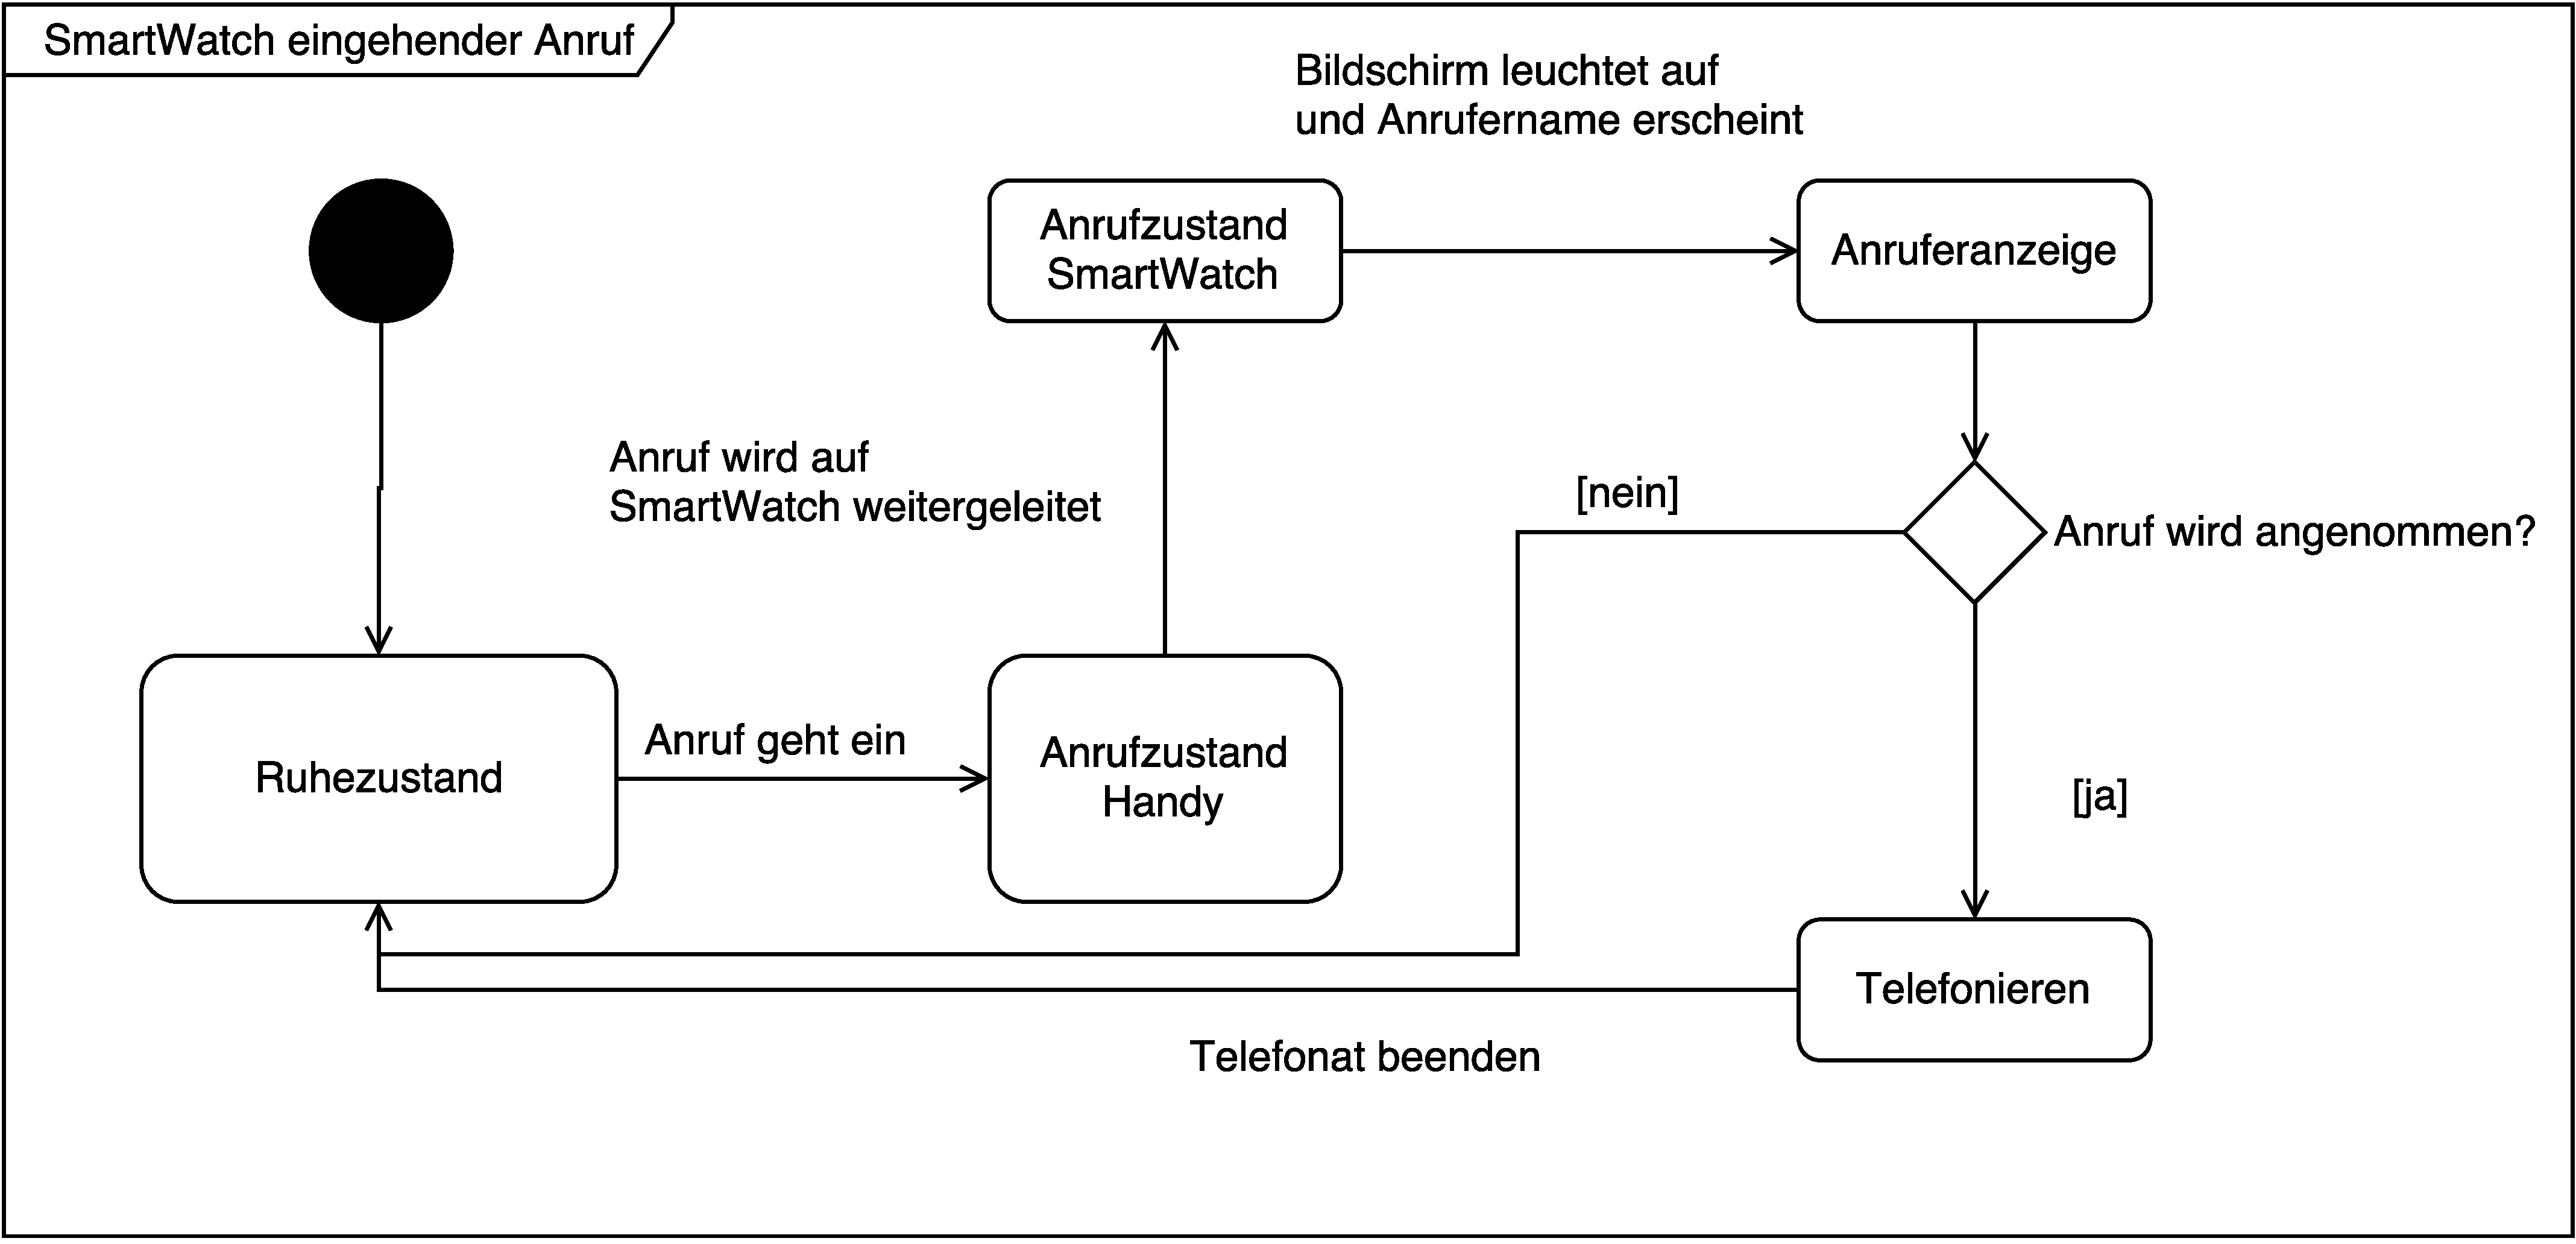
\includegraphics[width=\textwidth]{img/stateAnrufEingehend}
\caption[State Diagram: eingehender Anruf]{Verhalten der SmartWatch bei eineM eingehenden Anruf.}
\label{fig:stateAnrufEingehend}
\end{figure}
Als Nächstes wird das Verhalten der \textit{SmartWatch} bei einem \textit{eingehenden Anruf} näher betrachtet (Abb. \ref{fig:stateAnrufEingehend}). Zunächst befinden sich sowohl \textit{Handy} als auch \textit{Uhr} im \textit{Ruhezustand}. Wenn ein \textit{Anruf} eingeht, wechselt zuerst das \textit{SmartPhone} in den \textit{Anrufzustand} und gibt ein Signal an die \textit{Uhr} weiter. Sobald die \textit{Uhr} das Signal empfängt, wechselt auch sie in einen \textit{Anrufzustand}. Dabei wird die Bildschirmbeleuchtung aktiviert und die \textit{Anruferanzeige} eingeblendet. Diese \textit{Anzeige} ermöglicht es dem Benutzer zu wählen, ob er den Anruf entgegennehmen will oder nicht. Sollte er den Anruf annehmen, wechselt die \textit{SmartWatch} in den Zustand \textit{Telefonieren} und aktiviert das interne \textit{Mikrophon}. Sobald der Anruf beendet wird, kehren \textit{Telefon} und \textit{Uhr} in den \textit{Ruhezustand} zurück.\\
\begin{figure}[h]
\centering\
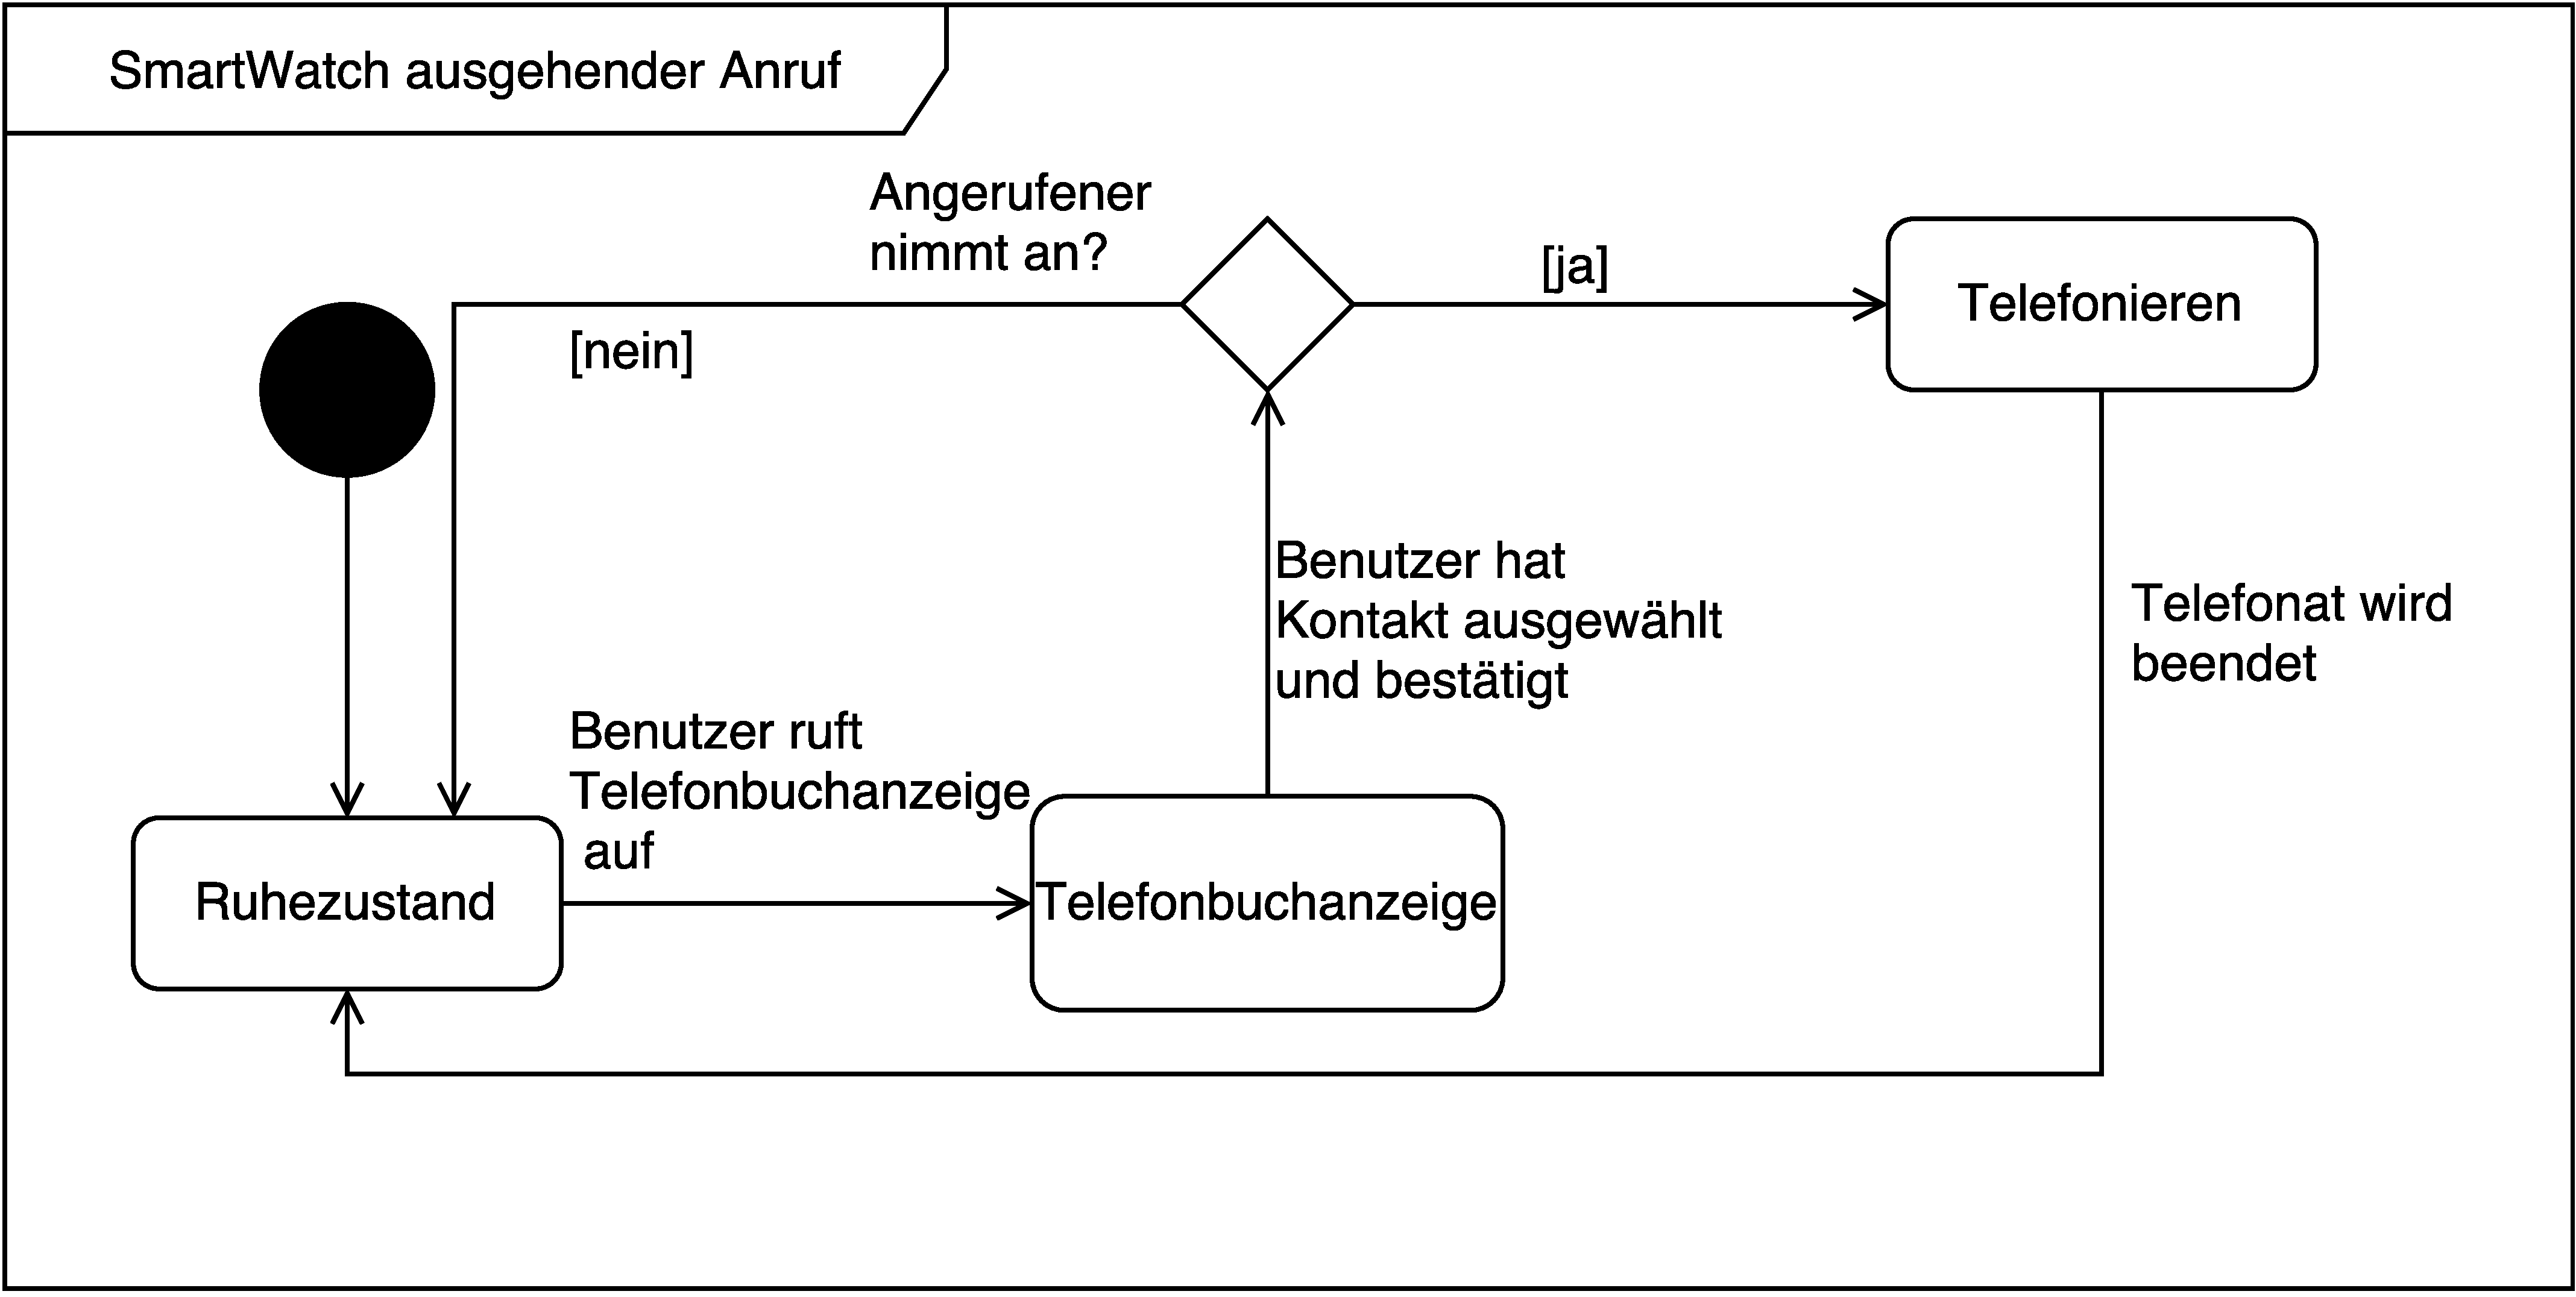
\includegraphics[width=\textwidth]{img/stateAnrufAusgehend}
\caption[State Diagram: ausgehender Anruf]{Verhalten der SmartWatch beim Tätigen eines Anrufs.}
\label{fig:stateAnrufAusgehend}
\end{figure}
Die von uns entwickelte \textit{SmartWatch} soll nicht nur in der Lage sein Anrufe anzunehmen, sondern auch \textit{Anrufe zu tätigen} (Abb. \ref{fig:stateAnrufAusgehend}). Auch hier wird wieder davon ausgegangen, dass sich beide Geräte im \textit{Ruhezustand} befinden. Beendet wird dieser durch das Aufrufen der \textit{Telefonbuchanzeige} auf der \textit{SmartWatch}. Sobald der \textit{Benutzer} einen \textit{Kontakt} aus dem Telefonbuch des \textit{SmartPhones} über die \textit{SmartWatch} gewählt hat, wird die \textit{Anruffunktionalität} eingeleitet. Sollte der Angerufene das Telefonat annehmen, wird auch hier in den Zustand \textit{Telefonieren} gewechselt. Dabei verhält sich die \textit{SmartWatch} genauso wie bei einem \textit{eingehenden Anruf}. Nach Beendigung des Gesprächs wechseln beide Geräte wieder in den \textit{Ruhezustand}.